\subtop{Binärbäume}{-1.45}\\
Die Tiefe eines Knotens ($depth(v)$) ist der Abstand von der Wurzel bis $v$.\\
Der \textit{Divide and Conquer}-Ansatz wird verwendet, um ein geradliniges Gitterlayout für geradlinige Repräsentationen zu finden. Dies funktioniert für Binärbäume wie folgt:
\begin{enumerate}[itemsep=-1pt]
	\item Bestimmung des Teillayouts für $T_l(v)$
	\item Bestimmung des Teillayouts für $T_r(v)$
	\item Zusammenfügen zu Gesamtlayouts
\end{enumerate}
\subsection{Baumdurchläufe}
Es gibt drei Arten von Baumduchläufen:
\begin{enumerate}[itemsep=-1pt]
	\item Preorder
	\item Inorder
	\item Postorder
\end{enumerate}
\begin{description}[itemsep=-1pt]
	\item[Ein Gitterlayout] hat ausschließlich ganzzahlige Koordinaten
	\item[Geradlinige Repräsentationen] sind Standardrepräsentationen mit geraden Kanten
	\item[Ein Layout ist vollatändig bestimmt,] wenn  für jeden Konten $v\in V$ eine $x$-Koordinate ($x(v)$) und eine $y$-Koordinate ($y(v)$) gegeben sind.
\end{description}
\subsection{Definition eines Gitterlayouts}
Für jeden Knoten ist der Punkt im Layout folgendermaßen definiert:
\begin{eqnarray*}
	x(v_i)&= & i\\
	y(v_i)& = & -depth(v_i)
\end{eqnarray*}
Dieses Layout ist \textit{abwärts}, \textit{kreuzungsfrei} und kann in Linearzeit bestimmt werden.\\
\example{Inorder-Layout}{\ \\\vspace*{-2\baselineskip}
	\usetikzlibrary{positioning,arrows}

\begin{tikzpicture}[node distance=1cm,scale=0.75]

\node (0) at (0,0) {\begin{tikzpicture}[every node/.style={draw,circle},scale=0.75]
\node[draw=none,color=blue] (l0) at (3,0) {\scriptsize 0};
\node[draw=none,color=blue] (l1) at (3,-1) {\scriptsize 1};
\node[draw=none,color=blue] (l2) at (3,-2) {\scriptsize 2};
\node[draw=none,color=blue] (l3) at (3,-3) {\scriptsize 3};

\node[fill=white] (1) at (0,0) {4};
\draw[dashed,color=blue](1)--++(l0);
\node[fill=white] (2) at (-1,-1) {3};
\draw[dashed,color=blue](2)--++(l1);
\node[fill=white] (3) at (1,-1) {6};
\node[fill=white] (4) at (-2,-2) {1};
\draw[dashed,color=blue](4)--++(l2);
\node[fill=white] (5) at (-1,-3) {2};
\draw[dashed,color=blue](5)--++(l3);
\node[fill=white] (6) at (0,-2) {5};
\node[fill=white] (7) at (2,-2) {7};

\foreach \x/\y in {1/2,1/3,2/4,4/5,3/6,3/7}{
	\draw[-](\x)--(\y);
}
\end{tikzpicture}};

\node (1) [right=of 0] {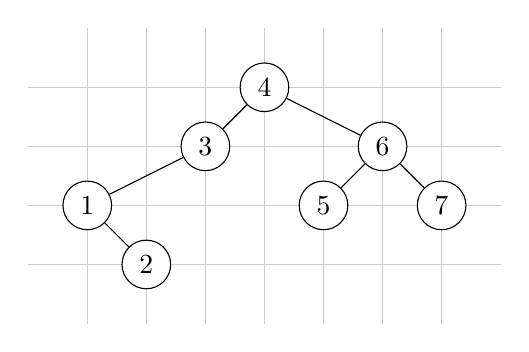
\begin{tikzpicture}[every node/.style={draw,circle},scale=0.75]
\foreach \x in {1,...,7}
	\draw[color=black!20](\x,1)--(\x,-4);
\foreach \y in {0,...,3}
	\draw[color=black!20](0,-\y)--(8,-\y);
\foreach[count=\c] \y in {2,3,1,0,2,1,2}
	\node[fill=white] (\c) at (\c,-\y) {\c};
\foreach \x/\y in {1/2,1/3,3/4,4/6,5/6,6/7}
	\draw[-](\x)--(\y);
\end{tikzpicture}};

\draw[->,>=latex,very thick](0)--(1);
\end{tikzpicture}
}
\example{Preorder-Layout}{\ \\\vspace*{-2\baselineskip}
	\usetikzlibrary{positioning,arrows}

\begin{tikzpicture}[node distance=1cm,scale=0.75]

\node (0) at (0,0) {\begin{tikzpicture}[every node/.style={draw,circle},scale=0.75]
\node[draw=none,color=blue] (l0) at (3,0) {\scriptsize 0};
\node[draw=none,color=blue] (l1) at (3,-1) {\scriptsize 1};
\node[draw=none,color=blue] (l2) at (3,-2) {\scriptsize 2};
\node[draw=none,color=blue] (l3) at (3,-3) {\scriptsize 3};

\node[fill=white] (1) at (0,0) {1};
\draw[dashed,color=blue](1)--++(l0);
\node[fill=white] (2) at (-1,-1) {2};
\draw[dashed,color=blue](2)--++(l1);
\node[fill=white] (3) at (1,-1) {5};
\node[fill=white] (4) at (-2,-2) {3};
\draw[dashed,color=blue](4)--++(l2);
\node[fill=white] (5) at (-1,-3) {4};
\draw[dashed,color=blue](5)--++(l3);
\node[fill=white] (6) at (0,-2) {6};
\node[fill=white] (7) at (2,-2) {7};

\foreach \x/\y in {1/2,1/3,2/4,4/5,3/6,3/7}{
	\draw[-](\x)--(\y);
}
\end{tikzpicture}};

\node (1) [right=of 0] {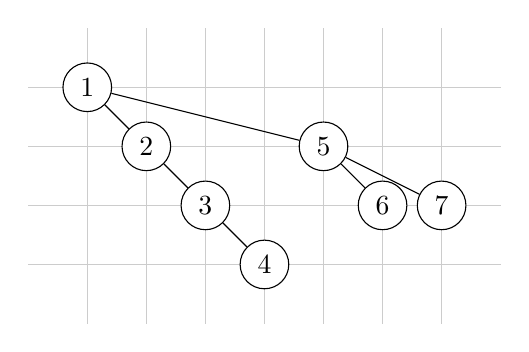
\begin{tikzpicture}[every node/.style={draw,circle},scale=0.75]
\foreach \x in {1,...,7}
	\draw[color=black!20](\x,1)--(\x,-4);
\foreach \y in {0,...,3}
	\draw[color=black!20](0,-\y)--(8,-\y);
\foreach[count=\c] \y in {0,1,2,3,1,2,2}
	\node[fill=white] (\c) at (\c,-\y) {\c};
\foreach \x/\y in {1/2,2/3,3/4,1/5,5/6,5/7}
	\draw[-](\x)--(\y);
\end{tikzpicture}};

\draw[->,>=latex,very thick](0)--(1);
\end{tikzpicture}
}
\topbreak
\vspace*{-1.5\baselineskip}
\begin{description}
	\item[Nachteile:]\ \\\vspace*{-\baselineskip}
		\begin{enumerate}[itemsep=-1pt]
			\item Breite $=n-1$
			\item Kantenlänge $\BigO(n)$
			\item Knoten sind nicht zentriert über Nachfolgern
		\end{enumerate}
\end{description}
Problem $1$ und $2$ können durch Berechnung relativer Koordinaten behoben werden:
\begin{itemize}[itemsep=-1pt]
	\item Berechnung der Koordinaten der Teilbäume getrennt
	\item Zusammenlegen der Layouts, sodass die \textit{umgebenden Rechtecke} Abstand $2$ oder $3$ haben
	\item Elterknoten wird zentriert über den Nachfolgern platziert (bzw. eins weiter nach rechts/links, wenn es wichtig ist, um welchen Nachfolger es sich handelt)
	\item[$\Rightarrow$] immer noch in Linearzeit bestimmbar, aber immer noch \textbf{zu breit}
		\begin{itemize}[itemsep=-1pt]
			\item[$\Rightarrow$] verwenden von \textbf{Konturen} statt Rechtecken:\\
			Platzieren der Teilbäume so, dass der minimale horizontale Abstand zweier Knoten de gleichen TIefe $2$ (bzw. $3$) ist
		\end{itemize}
\end{itemize}
\subsubsection{Bestimmung eines Layouts mithilfe von Konturen}
\begin{itemize}[itemsep=-1pt]
	\item Abstand zwischen zwei Knoten mit gleicher Tiefe ist zwei (drei, falls Teilbaumwurzeln sonst ungeraden Abstand haben)
	\item zur Bestimmung in Linearzeit (Bestimmung pro Knoten):
		\begin{enumerate}
			\item Berechnung des $x$-Offsets (relative Position zum Vorgänger)
			\item Speichern der linken und rechten Kontur seines Teilbaumes als eine einfach verkettete Liste
		\end{enumerate}
	\item Algorithmus von \textit{Reingold und Tilford} arbeitet in zwei Schritten:
		\begin{enumerate}
			\item \textit{postorder}: zur Bestimmung von Konturen und $x$-Offsets\\
			\begin{minipage}{0.43\textwidth}
				\usetikzlibrary{positioning,patterns}
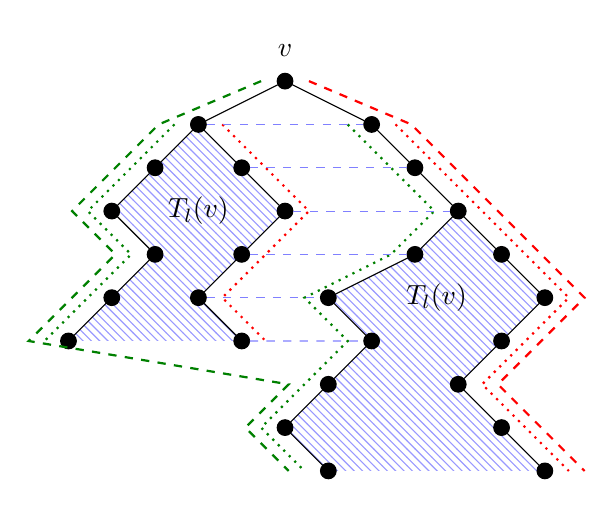
\begin{tikzpicture} [every node/.style={draw,circle,fill},node distance=0.2cm,scale=0.55]

\def\s{0.6}

\fill[pattern color=blue!40,pattern=north west lines](-2,1)--(-4,-1)--(-3,-2)--(-5,-4)--(-1,-4)--(-2,-3)--(0,-1);
\fill[pattern color=blue!40,pattern=north west lines](4,-1)--(3,-2)--(1,-3)--(2,-4)--(0,-6)--(1,-7)--(6,-7)--(4,-5)--(6,-3);

\node[scale=\s] (v1) at (0,2) {};
\node[scale=\s] (v2) at (-2,1) {};
\node[scale=\s] (v8) at (2,1) {};
\node[scale=\s] (v3) at (-3,0) {};
\node[scale=\s] (v15) at (-1,0) {};
\node[scale=\s] (v4) at (-4,-1) {};
\node[scale=\s] (v23) at (0,-1) {};
\node[scale=\s] (v5) at (-3,-2) {};
\node[scale=\s] (v24) at (-1,-2) {};
\node[scale=\s] (v25) at (-2,-3) {};
\node[scale=\s] (v16) at (-1,-4) {};
\node[scale=\s] (v6) at (-4,-3) {};
\node[scale=\s] (v7) at (-5,-4) {};
\node[scale=\s] (v9) at (3,0) {};
\node[scale=\s] (v21) at (4,-1) {};
\node[scale=\s] (v10) at (5,-2) {};
\node[scale=\s] (v11) at (6,-3) {};
\node[scale=\s] (v17) at (3,-2) {};
\node[scale=\s] (v18) at (1,-3) {};
\node[scale=\s] (v19) at (2,-4) {};
\node[scale=\s] (v20) at (1,-5) {};
\node[scale=\s] (v26) at (0,-6) {};
\node[scale=\s] (v27) at (1,-7) {};
\node[scale=\s] (v22) at (5,-4) {};
\node[scale=\s] (v12) at (4,-5) {};
\node[scale=\s] (v13) at (5,-6) {};
\node[scale=\s] (v14) at (6,-7) {};
\draw (v1) -- (v2) -- (v3) -- (v4) -- (v5) -- (v6) -- (v7);
\draw (v1) -- (v8) -- (v9) -- (v21) -- (v10) -- (v11) -- (v22) -- (v12) -- (v13) -- (v14);
\draw (v2) -- (v15) -- (v23) -- (v24) -- (v25) -- (v16);
\draw (v21) -- (v17) -- (v18) -- (v19) -- (v20) -- (v26) -- (v27);
\foreach \x in {1,...,9,17,18,19,20,21,26,27}{
	\coordinate[left=of v\x] (cl\x);
%	\node[draw=none,fill=none] at (cl\x) {\x};
}
\foreach \x in {1,2,8,9,10,11,12,13,14,15,16,21,22,23,24,25}{
	\coordinate[right=of v\x] (cr\x);
%	\node[draw=none,fill=none] at (cr\x) {\x};
}

\foreach \x in {2,...,7,20,26,27}{
	\coordinate[left=of cl\x] (ccl\x);
%	\node[draw=none,fill=none] at (ccl\x) {\x};
}
\foreach \x in {8,9,10,11,12,13,14,21,22}{
	\coordinate[right=of cr\x] (ccr\x);
%	\node[draw=none,fill=none] at (ccr\x) {\x};
}
\path[dotted,color=green!50!black,draw,thick](cl2)--(cl4)--(cl5)--(cl7);
\path[dashed,color=green!50!black,draw,thick](cl1)--(ccl2)--(ccl4)--(ccl5)--(ccl7)--(ccl20)--(ccl26)--(ccl27);
\path[dotted,color=green!50!black,draw,thick](cl8)--(cl21)--(cl17)--(cl18)--(cl19)--(cl26)--(cl27);
\path[dotted,color=red,draw,thick](cr2)--(cr15)--(cr23)--(cr25)--(cr16);
\path[dotted,color=red,draw,thick](cr8)--(cr11)--(cr12)--(cr14);\path[dashed,color=red,draw,thick](cr1)--(ccr8)--(ccr11)--(ccr12)--(ccr14);

\node[draw=none,fill=none] (tl) at (-2,-1) {$T_l(v)$};
\node[draw=none,fill=none] (tl) at (3.5,-3) {$T_l(v)$};

\node[draw=none,fill=none,yshift=-0.2cm] (v)[above=of v1] {$v$};

\foreach \x/\y in {2/8,15/9,23/21,24/17,25/18,16/19}{
	\draw[dashed,color=blue!50](v\x)--(v\y);
}

\end{tikzpicture}
			\end{minipage}
			\begin{minipage}{0.47\textwidth}
				\begin{itemize}[itemsep=-1pt]
					\item[] 
					\item Abarbeiten von $\tl$ und $\tr$
					\item Absteigen in den Konturen beider Teilbäume parallel, bis die Konturen des niedrigeren Teilbaums endet
					\item linke (rechte) Kontur von $T(v)$ besteht aus $v$, der linken (rechten) Kontur von $T_l(v)$ ($T_r(v)$) und dem (falls vorhanden) linken (rechten) Kontur von $T_r(v)$ ($T_l(v)$)
					\item Bestimmen des Mindestabstandes $d\geq 2$ der Nachfolger von $v$ aus den $x$-Offsets der rechten Kontur von $T_l(v)$ und der linken Kontur von $T_r(v)$
					\item Erhöhen von $d_v$ um $1$, falls ungerade
					\item Setzten des $x$-Offsets der Nachfolger von $v$ (wenn vorhanden) auf $-\frac{d_v}{2}$ bzw. $+\frac{d_v}{2}$
				\end{itemize}
			\end{minipage}
			\item[2.] \textit{preorder}: Kalkulation der $x$-Koordinaten mithilfe des Zusammennehmens der $x$-Offsets
				\begin{itemize}
					\item Bearbeitung von $T(v)$: $x$ ist die Koordinate des Vorgängers (oder $x=0$, falls $v$ die Wurzel ist)
					\item $x(v)  = x+ x-Offset(v)$
					\item Algorithmus von Reingold/Tilford (in Linearzeit) berechnet:
						\begin{itemize}
							\item geradliniges Gitterlayout, das tiefengeschichtet und kreuzungsfrei ist
							\item Knoten mit selber Tiefe haben Abstand $\geq 2$
							\item Knoten sind über Nachfolgern zentriert
							\item linke/rechte Nachfolger liegen strikt links/rechts von ihrem Vorgänger
							\item identische Teilbäume sind gleich ausgelegt
						\end{itemize}
						$\Rightarrow$ Binärbaumlayout*
				\end{itemize}
		\end{enumerate} 
\end{itemize}

\topbreak
* Das Layout ist nicht unbedingt Platzoptimal:\\
\begin{minipage}{0.45\textwidth}
	\usetikzlibrary{positioning,patterns}
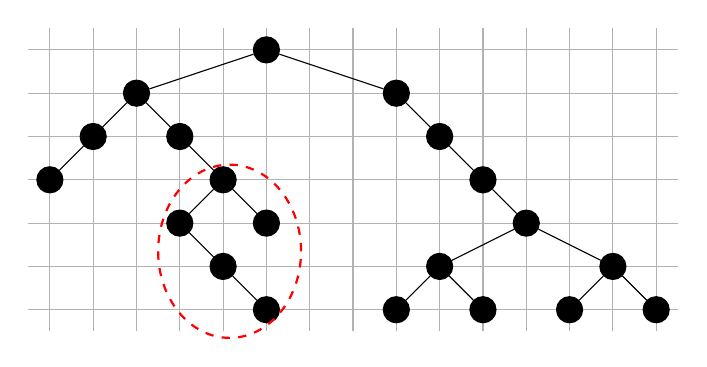
\begin{tikzpicture} [every node/.style={draw,circle,fill},node distance=0.2cm,scale=0.55]
\def\ymin{-6}
\def\xmin{-5}
\def\ymax{0}
\def\xmax{9}

\foreach \x in {\xmin,...,\xmax}
	\draw[color=black!30](\x,\ymin-0.5)--(\x,\ymax+0.5);
\foreach \y in {\ymin,...,\ymax}
	\draw[color=black!30](\xmin-0.5,\y)--(\xmax+0.5,\y);


\node (v1) at (0,0) {};
\node (v2) at (-3,-1) {};
\node (v19) at (3,-1) {};
\node (v20) at (-2,-2) {};
\node (v3) at (-4,-2) {};
\node (v5) at (-1,-3) {};
\node (v4) at (-5,-3) {};
\node (v9) at (0,-4) {};
\node (v6) at (-2,-4) {};
\node (v7) at (-1,-5) {};
\node (v8) at (0,-6) {};
\node (v10) at (4,-2) {};
\node (v11) at (5,-3) {};
\node (v14) at (6,-4) {};
\node (v15) at (4,-5) {};
\node (v12) at (8,-5) {};
\node (v16) at (3,-6) {};
\node (v17) at (5,-6) {};
\node (v13) at (7,-6) {};
\node (v18) at (9,-6) {};

\foreach \x/\y in {1/2,2/3,3/4,2/20,20/5,5/6,6/7,7/8,5/9,1/19,19/10,10/11,11/14,14/12,14/15,15/16,15/17,12/13,12/18}
	\draw (v\x)edge (v\y);

\draw[color=red,thick, dashed] (-0.85,-4.65) ellipse (1.65 and 2);

\end{tikzpicture}
\end{minipage}\hfill
\begin{minipage}{0.45\textwidth}
	\usetikzlibrary{positioning,patterns}
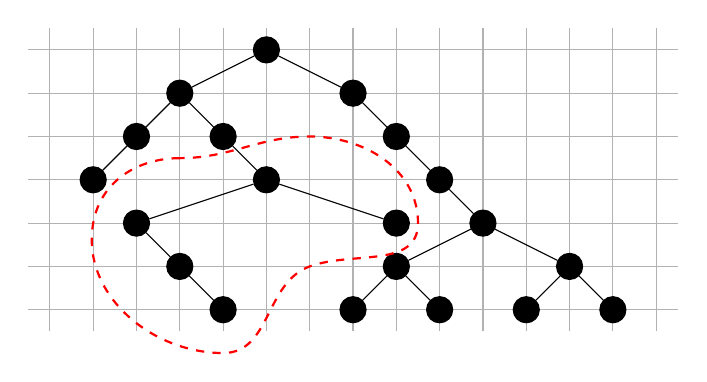
\begin{tikzpicture} [every node/.style={draw,circle,fill},node distance=0.2cm,scale=0.55]
\def\ymin{-6}
\def\xmin{-5}
\def\ymax{0}
\def\xmax{9}

\foreach \x in {\xmin,...,\xmax}
	\draw[color=black!30](\x,\ymin-0.5)--(\x,\ymax+0.5);
\foreach \y in {\ymin,...,\ymax}
	\draw[color=black!30](\xmin-0.5,\y)--(\xmax+0.5,\y);


\node (v1) at (0,0) {};
\node (v2) at (-2,-1) {};
\node (v19) at (2,-1) {};
\node (v20) at (-1,-2) {};
\node (v3) at (-3,-2) {};
\node (v5) at (0,-3) {};
\node (v4) at (-4,-3) {};
\node (v9) at (3,-4) {};
\node (v6) at (-3,-4) {};
\node (v7) at (-2,-5) {};
\node (v8) at (-1,-6) {};
\node (v10) at (3,-2) {};
\node (v11) at (4,-3) {};
\node (v14) at (5,-4) {};
\node (v15) at (3,-5) {};
\node (v12) at (7,-5) {};
\node (v16) at (2,-6) {};
\node (v17) at (4,-6) {};
\node (v13) at (6,-6) {};
\node (v18) at (8,-6) {};

\foreach \x/\y in {1/2,2/3,3/4,2/20,20/5,5/6,6/7,7/8,5/9,1/19,19/10,10/11,11/14,14/12,14/15,15/16,15/17,12/13,12/18}
	\draw (v\x)edge (v\y);

\draw[color=red,thick, dashed](-2,-2.5)to[out=180,in=80](-4,-4)to[out=260,in=180](-1,-7)to[out=0,in=200](1,-5)to[out=20,in=270](3.5,-4)to[out=90,in=0](1,-2)to[out=180,in=0] (-2,-2.5);

\end{tikzpicture}
\end{minipage}
\subsubsection{Die Breitenminimierung von Binärbäumen ist $\mathcal{NP}$-schwer.}
\ProofIdea
\textit{Bemerkung:} Das Problem ist in $\mathcal{P}$, falls keine ganzzahligen Koordinaten (Gitterlayout) erforderlich sind.\\
\textit{Allgemeine Idee:}\\
\usetikzlibrary{intersections,arrows}
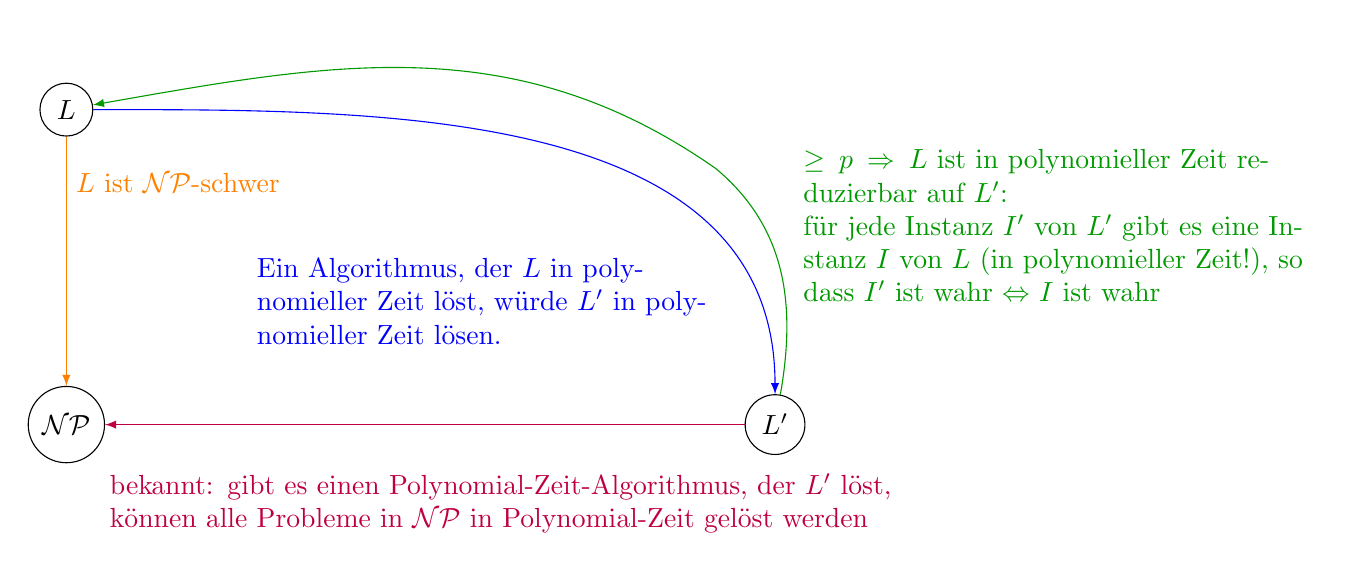
\begin{tikzpicture}[]

\node[draw,circle] (L) at (0,0) {$L$};
\node[draw,circle] (L') at (9,-4) {$L'$};
\node[draw,circle] (NP) at (0,-4) {$\mathcal{NP}$};

\draw[->,>=latex,color=blue](L)to[out=0,in=90] node[text width=6cm,left,xshift=2.5cm,yshift=-2cm]{Ein Algorithmus, der $L$ in polynomieller Zeit l\"ost, w\"urde $L'$ in polynomieller Zeit l\"osen.}(L');
\draw[->,>=latex,color=green!60!black](L')to[out=80,in=320](8.25,-0.75) to[out=145,in=10] node[text width=6.5cm,right,xshift=4.75cm,yshift=-2cm]{$\geq p \Rightarrow L$ ist in polynomieller Zeit reduzierbar auf $L'$:\\ f\"ur jede Instanz $I'$ von $L'$ gibt es eine Instanz $I$ von $L$ (in polynomieller Zeit!), so dass $I'$ ist wahr $\Leftrightarrow$ $I$ ist wahr}(L);
\draw[->,>=latex,color=orange](L)to node[text width=3.5cm,right,xshift=0cm,yshift=1cm]{$L$ ist $\mathcal{NP}$-schwer}(NP);
\draw[->,>=latex,color=purple](L')to[out=180,in=0] node[text width=10cm,below,xshift=1cm,yshift=-0.5cm]{bekannt: gibt es einen Polynomial-Zeit-Algorithmus, der $L'$ löst, können alle Probleme in $\mathcal{NP}$ in Polynomial-Zeit gelöst werden}(NP);
\end{tikzpicture}\\
Hier wird gezeigt, dass sogar für feste Werte ($\mathcal{W}=24$) das Problem in $\mathcal{NP}$ liegt. Das Problem ist sicher in $\mathcal{NP}$, da sich jedes gegebene Layout auf die Eigenschaften eines Binärbaumes und die Breite prüfen lässt.\\
\textit{Ablauf des Beweises:}
	\begin{itemize}
		\item Reduzierung von $3$-SAT auf Binärbaum mit minimaler Breite mithilfe von $F=C_1 \wedge \dots \wedge C_m$ als $3$-SAT-Formel mit
			\begin{itemize}
				\item Klauseln $C_i=y_{i,1}\vee y_{i,2}\vee y_{i,3}$
				\item Literalen $y_{i,j}\in\{x_1,\dots,x_n,\overline{x_1},\dots,\overline{x_n}\}$
			\end{itemize}
		\item Konstruktion der Instanz $T(F)$ für das Layoutproblem, die genau dann ein Layout mit Breite $\mathcal{W}\leq 24$ hat, falls $F$ erfüllbar ist
		\item Erzeugung von Teilbäumen für Variablen, Literale und Klauseln
		\item Teilbäume der drei in der Klausel $C_i$ auftretenden Literale werden zu $T(C_i)$ zusammengefügt (mithilfe von einer ausreichend langen Kette von Knoten, die beim mittleren Literal eingefügt wird und an der Wurzel des nächsten Baumes endet)
		\item Beweis, dass falls $F$ gilt auch $T(F)$ gilt und falls $F$ nicht gilt auch $T(F)$ nicht gilt
	\end{itemize}
\topbreak
\subsection{Radiales Layout}
\begin{minipage}{0.4\textwidth}
	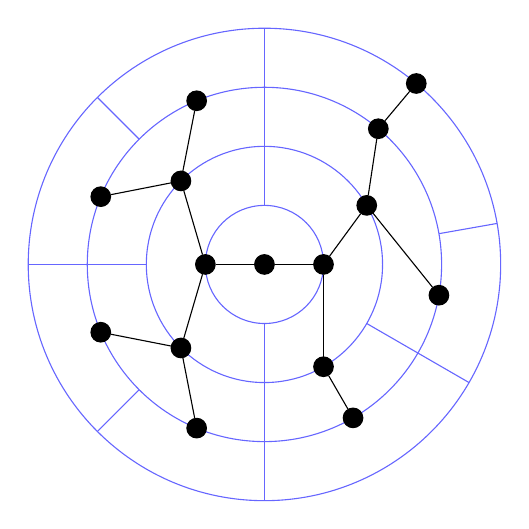
\begin{tikzpicture}[]

\def\r{0.75}
\def\a{4}

\foreach \x in {1,...,\a}
	\draw[color=blue!60] (0,0) circle (\x*\r);

\node[draw,fill,circle,scale=0.75](0)at(0,0){};

\foreach[count=\i,evaluate=\i as \angle using (\i-1)*360/2] \text in {1,2}
    \node[draw,circle,scale=0.75,fill] (1-\i) at (\angle:\r) {};

\draw[color=blue!60](0,\r)--(0,\a*\r);
\draw[color=blue!60](0,-\r)--(0,-\a*\r);
\draw[color=blue!60](-2*\r,0)--(-\a*\r,0);

\foreach[count=\i,evaluate=\i as \angle using (\i-1)*360/4] \text in {1,2}{
	\node[draw,circle,scale=0.75,fill] (2-\i) at (\angle-5*360/8:2*\r) {};
}

\foreach[count=\i,evaluate=\i as \angle using (\i-1)*360/8] \text in {1,2,3,4}{
	\node[draw,circle,scale=0.75,fill] (3-\i) at (\angle-11*360/16:3*\r) {};
}

\foreach[count=\i,evaluate=\i as \angle using (\i-1)*360/4] \text in {1,2}{
	\coordinate (c1-\text) at (\angle-10*360/16:3*\r) {};
	\coordinate (c2-\text) at (\angle-10*360/16:4*\r) {};
}
\draw[color=blue!60](c1-1)--(c2-1);
\draw[color=blue!60](c1-2)--(c2-2);

\node[draw,circle,scale=0.75,fill] (2-4) at (30:2*\r) {};
\node[draw,circle,scale=0.75,fill] (2-3) at (300:2*\r) {};

\coordinate (1) at (330:2*\r) {};
\coordinate (2) at (330:4*\r) {};
\draw[color=blue!60](1)--(2);

\coordinate (1) at (10:3*\r) {};
\coordinate (2) at (10:4*\r) {};
\draw[color=blue!60](1)--(2);

\node[draw,circle,scale=0.75,fill] (3-5) at (300:3*\r) {};
\node[draw,circle,scale=0.75,fill] (3-6) at (350:3*\r) {};
\node[draw,circle,scale=0.75,fill] (3-7) at (50:3*\r) {};
\node[draw,circle,scale=0.75,fill] (4-7) at (50:4*\r) {};

\foreach \x/\y in {0/1-1,0/1-2,1-1/2-3,1-1/2-4,1-2/2-1,1-2/2-2,2-1/3-1,2-1/3-2,2-2/3-3,2-2/3-4,2-3/3-5,2-4/3-6,2-4/3-7,3-7/4-7}
	\draw(\x)--(\y);
\end{tikzpicture}
\end{minipage}\hfill
\begin{minipage}{0.6\textwidth}
	\begin{itemize}[itemsep=-1pt]
		\item der Radius entspricht der Tiefe des Knotens
		\item rekursive Zuweisung der Position jeden Knotens, mit dem ihm noch verbleibenden Kreisteil
		\item für ein kreuzungsfreies Layout wird der für die Rekursion verfügbare Platz durch die Tangente der Teilbaumwurzel beschränkt
		\item \algo{Radiales Baumlayout}{\begin{algorithm}[H]
	\SetAlgoVlined
	\SetKwProg{Fn}{Function}{}{end}
	\SetKwFunction{po}{postorder}
	\SetKwFunction{pr}{preorder}
	\KwIn{Binärbaum $T=(V,E)$ mit Wurzel $R\in V$}
	\KwData{Anzahl $n_v$ der Knoten in Teilbaum $T(v),v\in V$}
	\KwOut{Polarkoordinaten $p_v=(d_v,\alpha_v),v\in V$}
	\BlankLine
	\Fn{\po{vertex $v$}}{
		$n_v\leftarrow 1;$\\
		\ForEach{Nachfolger $w$ von $v$}{
			\post($w$);\\
			$n_v\leftarrow n_v+n_w$;
		}
	}
	\Fn{\pr{vertex $v$, double $t$,$\alpha_{min}$,$\alpha_{max}$}}{
			$d_v\leftarrow t;$\\
			$\alpha_v\leftarrow \frac{\alpha_{min}+\alpha_{max}}{2};$\\
			\If{$t>0$}{
				$\alpha_{min}\leftarrow \max\{\alpha_{min},\alpha_{v}-\arccos\frac{t}{t+1}\}$;\\
				$\alpha_{max}\leftarrow \min\{\alpha_{max},\alpha_{v}+\arccos\frac{t}{t+1}\}$;
			}
			$left\leftarrow\alpha_{min}$;\\
			\ForEach{Nachfolger $w$ von $v$}{
				$right\leftarrow left+\frac{n_w}{n_v-1}\cdot (\alpha_{max}-\alpha_{min})$;\\
				\pre($w$,$t+1$,$left$,$right$);\\
				$left\leftarrow right$;
			}
		}
	\Begin{
		\post($r$);\\
		\pre($r,0,0,2\pi$);
	}
\end{algorithm}
} (berechnet in linearer Zeit ein kreuzungsfreies Layout)
	\end{itemize}
	\centering{\usetikzlibrary{intersections}
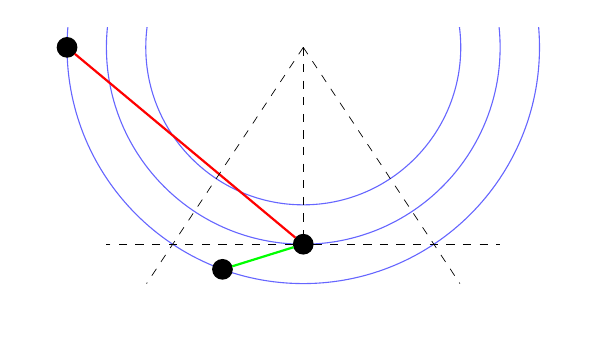
\begin{tikzpicture}[rotate=270]

\newcommand\ZeichneGerade[6]{% 
  \coordinate (Punkt1) at (#1,#2); 
  \coordinate (Punkt2) at (#3,#4); 
  \pgfmathsetmacro\m{(#4-#2)/(#3-#1)}% 
  \pgfmathsetmacro\n{#2-\m*#1}% 
  \draw[dashed,line width=0.25pt] plot[domain=#5:#6] (\x,{\m*\x+\n}); 
} 
%Syntax: \ZeichneGerade{x1}{y1}{x2}{y2}{anfang plotbereich}{ende plotbereich} 

\def\r{0.5}
\def\a{6}
\begin{scope}
\clip (-0.25,-\a*\r-0.5)rectangle(\r*\a+0.5,\r*\a+0.5);
\path[color=blue!60,draw,name path=c] (0,0) circle (4*\r);
\path[color=blue!60,draw,name path=c] (0,0) circle (5*\r);
\path[color=blue!60,draw,name path=c] (0,0) circle (6*\r);
\end{scope}
\node[draw,circle,scale=0.75,fill] (1) at (0:5*\r) {};
\node[draw,circle,scale=0.75,fill] (2) at (270:6*\r) {};
\node[draw,circle,scale=0.75,fill] (3) at (340:6*\r) {};

\draw[thick,color=red](1)--(2);
\draw[thick,color=green](1)--(3);

\draw[dashed](0,0)--(1);
\path[dashed,draw,name path=1](1)--++(0,-2.5);
\path[dashed,draw,name path=2](1)--++(0,2.5);

\ZeichneGerade{0}{0}{5*\r}{1.658}{0}{6*\r}
\ZeichneGerade{0}{0}{5*\r}{-1.658}{0}{6*\r}

\end{tikzpicture}}
\end{minipage}
